

%!TEX root = ../Notes.tex
\section{Normalness} 
\begin{definition}
	Let $(X,F_x)$ be a topological space. We say $X$ is \textbf{normal} if for every pair of disjoint closed sets $A,B \subseteq X$, there exist disjoint open sets $U,V\subseteq X$ such that $A \subseteq U$ and $B \subseteq V$. 
\end{definition}

On Homework 2, we proved that metric spaces are normal. 
\begin{example}
	Consider $\R$ with a topology $F$ defined by a basis of all sets of the form $(a,b)$ plus all sets of the form $(a,b)\cap \Q.$ This is known as the \textbf{rational topology}, and it is finer than the usual topology. As an exercise, you can prove that that this collection of sets really form the basis of a topology. (Use the basis lemma.) 
	
	We want to show that $(\R,F)$ is Hausdorff. This is easy, because $F$ contains the usual topology on on $\R$, which is Hausdorff. 
	
	Next, we will show that $(\R,F)$ is not normal. To see why, let $A=\R\setminus\Q.$ Then $A$ is closed, because $\Q$ is contained in $F$. Let $B=\{47\}.$ Suppose there exist $U,V \in F$ such that $A \subseteq U,$ and $B \subseteq V$. Then there exists $\epsilon>0$ such that $(47-\epsilon,47+\epsilon)\cap Q \subseteq V$. 
	
	Let $p \in (47-\epsilon,47+\epsilon)$ such that $p \not\in \Q.$ Then $p \in U$ because $p \not\in \Q$. So, there exists $\delta>0$ such that $(p-\delta,p+\delta) \subseteq U$. 
	
	Now, there must exist a point in $x \in (p-\delta,p+\delta)\cap((47-\epsilon,47+\epsilon) \cap \Q).$ But then $x \in U \cap V$, and so $U \cap V \neq \emptyset$. This proves that $(\R,F)$ is not a normal space. 
\end{example}

In particular, we have shown that a space can be Hausdorff but not normal. Under what conditions \emph{must} a Hausdorff space be normal?
\begin{lemma}
	If $(X,F_x)$ is Hausdorff and compact, then $X$ is normal. 
\end{lemma}
\setcounter{subfigure}{0} 
\begin{proof}
	{Comic-book style} 
	\begin{figure}
		[h!] 
		\begin{center}
			\subfigure[Let $A$ and $B$ be closed and disjoint sets.
			\newline Let $a\in A$.] {
			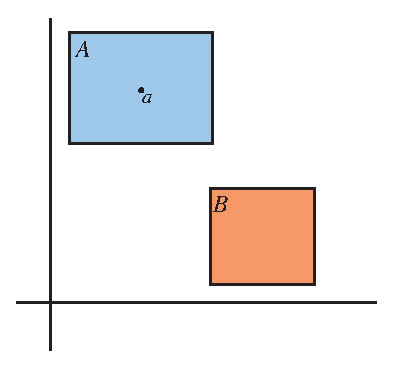
\includegraphics[width=210pt]{images/hausdorffness/hausdorff_comic_1}} \subfigure[Each point in $B$ can be separated from $a$ by an open set. This forms an open cover. Take a finite subcover.] {
			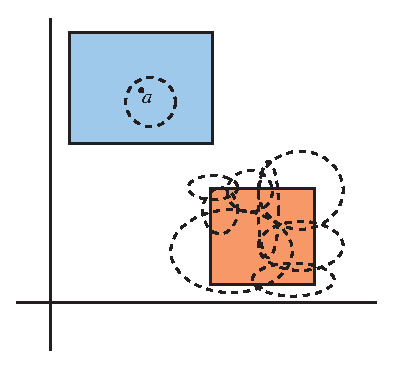
\includegraphics[width=210pt]{images/hausdorffness/hausdorff_comic_2}} 
		\end{center}
	\end{figure}
	\begin{figure}
		\begin{center}
			\subfigure[Repeat for each $a\in A$. This makes an open cover of $A$ and a lot of finite open covers of $B$.] {
			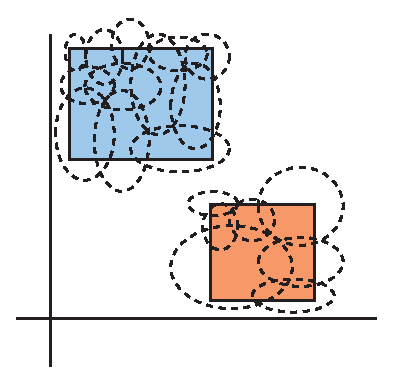
\includegraphics[width=210pt]{images/hausdorffness/hausdorff_comic_3}} \subfigure[Take the intersection of all of the covers of $B$. It's disjoint from the cover of $A$, so $A$ and $B$ are separated by open sets, so $X$ is normal.] {
			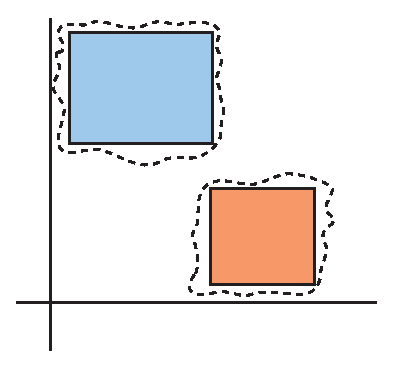
\includegraphics[width=210pt]{images/hausdorffness/hausdorff_comic_4}} 
		\end{center}
	\end{figure}
	\newpage 
\end{proof}
\vskip1cm

Now for the real proof. 
\begin{proof}
	Let $A$ and $B$ be disjoint closed subsets of $X$. Then $A$ and $B$ are compact because $X$ is compact. Let $a \in A$. For every $b \in B$, there exist open sets $U_b$ and $V_b$ such that $a \in U_b$ and $b \in V_b,$ and $U_b \cap V_b = \emptyset.$ Then $\{V_b \mid b \in B\}$ is an open cover of $B$. Since $B$ is compact, we can choose a finite subcover $\{V_{b_1},\ldots,V_{b_n}\}.$ Let $U_a=\cap_{i=1}^n U_{b_i}$. For every $a \in A$, $U_a \in F_x$ and $a \in U_a.$ Let $V_a=\cup_{i=1}^n V_{b_i}$. Then $B \subseteq V_a \in F_x$. 
	
	We claim that $U_a \cap V_a = \emptyset$ for all $a \in A$. To see why, note that $\left( \cap_{i=1}^n U_{b_i}\right) \cap \left( \cup_{i=1}^n V_{b_i} \right) = \emptyset$ because for all $i$, $U_{b_i} \cap V_{b_i}=\emptyset.$
	
	Now, $\{U_a \mid a \in A\}$ is an open cover of $A$. Since $A$ is compact, this cover has a finite subcover $\{U_{a_1},\ldots,U_{a_m}\}$. Now, $V=\cap_{i=1}^{m}V_{a_i}$ is open and $B \subseteq V$. For all $i=1,\ldots,m,$ $U_{a_i}\cap \left( \cap_{i=1}^m V_{a_i} \right) = \emptyset$ because for all $i=1,\ldots,m$, $U_{a_i} \cap V_{a_i}=\emptyset$. 
	
	Let $U=\cup_{i=1}^m U_{a_i} \in F_x$. Then $A \subseteq U$ and $U \cap V = \emptyset$ because $U_{a_i} \cap V_{a_i}=\emptyset$ for all $i$.
	
	Therefore, $X$ is normal. 
\end{proof}
\begin{theorem}
	Let $(X,F_X)$ be a compact and Hausdorff topological space. If $(Y,F_Y)$ is a topological space and $f : X \to Y$ is continuous, onto, and closed, then $(Y,F_Y)$ is compact and Hausdorff. 
\end{theorem}
\begin{proof}
	From previous notes, since $f$ is continuous and $X$ is compact, $Y$ is compact.
	
	So now consider Hausdorff:
	
	Let $p,q \in Y$ such that $p \neq q$. As $f$ is onto, $\exists \ a,b \in X$ such that $f(a) = p$ and $f(b) = q$. As $X$ is Hausdorff, $\{a\}$ and $\{b\}$ are closed. As $f$ is closed, $f(\{a\}) = \{p\}$ and $f(\{b\}) = \{q\}$ are closed. Therefore, as $f$ is continuous, $f^{-1}(\{p\})$ and $f^{-1}(\{q\})$ are closed, and are clearly disjoint.
	
	As $X$ is both compact and Hausdorff, it is also normal. So $\exists \ U,V \in F_X$ such that $f^{-1}(\{p\}) \subseteq U$, $f^{-1}(\{q\}) \subseteq V$, and $U \cap V = \emptyset$. As these sets are open, $A = U^c$ and $B = V^c$ are closed. As $f$ is closed, $f(A)$ and $f(B)$ are also closed, and hence $f(A)^c$ and $f(B)^c$ are open.
	
	Suppose that $p \in f(A)$. Then for some $x \in A$, $f(x) = p$. But then $x \in f^{-1}(\{p\}) \subseteq U = A^c$. So $x \in A \cap A^c$, which is a contradiction. So $p \in f(A)^c$, and by a similar argument, $q \in f(B)^c$.
	
	Now suppose that $c \in f(A)^c \cap f(B)^c$. So, as $f$ is onto, there exists some $d \in X$ such that $f(d) = c$. As $c \notin f(A)$, $d \notin A$, so $d \in U$. Similarly, as $c \notin f(B)$, $d \in V$. But then $d \in U \cap V = \emptyset$. This is a contradiction, so no such $c$ exists, and $f(A)^c \cap f(B)^c = \emptyset$.
	
	So $f(A)^c$ and $f(B)^c$ are disjoint open sets with $p \in f(A)^c$ and $q \in f(B)^c$. As such open sets exist for all $p,q \in Y$, $Y$ is Hausdorff.
	
	Therefore $Y$ is compact and Hausdorff, as desired. 
\end{proof}
